\section{Methods}
\label{sec:methods}

\subsection{Atrous Convolution for Dense Feature Extraction and Field-of-View Enlargement}
\label{sec:convnet-hole}
The use of DCNNs for semantic segmentation, or other dense prediction tasks, has been shown to be
simply and successfully addressed by deploying DCNNs in a fully convolutional fashion \cite{sermanet2013overfeat, long2014fully}.
 However, the repeated combination of max-pooling and striding
 at consecutive layers of these networks reduces significantly the spatial resolution of the
 resulting feature maps, typically by a factor of 32 across each direction in recent DCNNs.
 A partial remedy is to use `deconvolutional' layers as  in  \cite{long2014fully},
which however requires additional memory and time.
 
We advocate instead the use of atrous convolution, originally developed for the efficient computation of the
undecimated wavelet transform in the ``algorithme \`a trous'' scheme of
\cite{holschneider1989real} and used before in the DCNN context by
\cite{giusti2013fast, sermanet2013overfeat, papandreou2014untangling}.
This algorithm allows us to compute the responses of any layer at any desirable resolution.
It can be applied post-hoc, once a network has been trained, but can also be seamlessly integrated with training.

Considering one-dimensional signals first, the output $y[i]$ of atrous convolution \footnote{We follow the
standard practice in the DCNN literature and use non-mirrored filters in this
definition.} of a 1-D input signal $x[i]$ with a filter $w[k]$ of length $K$ is
defined as:
\begin{equation}
  y[i] = \sum_{k=1}^K x[i + r \cdot k] w[k].
\end{equation}
The \emph{rate} parameter $r$ corresponds to the stride with which we sample the
input signal. Standard convolution is a special case for rate $r = 1$.
See \figref{fig:hole} for illustration.

 \begin{figure}
  \begin{tabular}{c}
%  \includegraphics[width=0.5\linewidth]{fig/atrous2.pdf}
    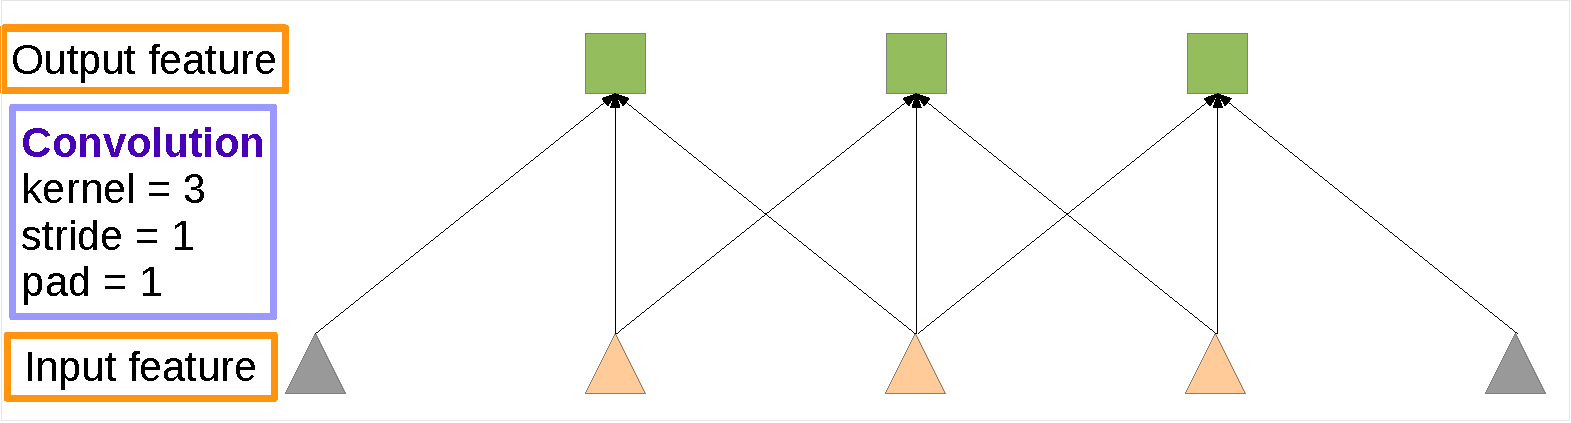
\includegraphics[width=0.9\linewidth]{fig/atrous_fig1.pdf} \\
    {\scriptsize (a) Sparse feature extraction} \\
    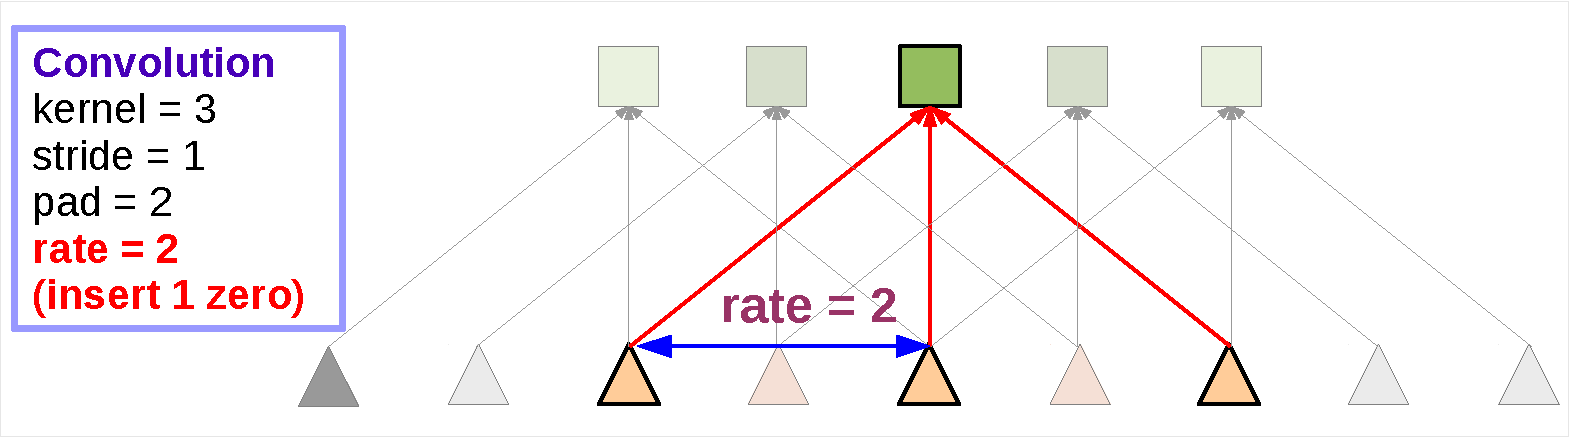
\includegraphics[width=0.9\linewidth]{fig/atrous_fig2.pdf} \\
    {\scriptsize (b) Dense feature extraction} \\
  \end{tabular}
  \caption{Illustration of atrous convolution in 1-D. (a) Sparse feature
    extraction with standard convolution on a low resolution input feature map.
    (b) Dense feature extraction with atrous convolution with rate $r = 2$,
    applied on a high resolution input feature map.}
  \label{fig:hole}
\end{figure}

We illustrate the algorithm's operation in 2-D through a simple example in \figref{fig:hole2d}: Given an image, we 
assume that we first have a downsampling operation that reduces the resolution by a factor of 2, and then perform  a 
convolution with a  kernel - here, the vertical Gaussian derivative. If one  implants the resulting 
feature map in the original image coordinates, we realize that we have obtained responses at only 1/4 of the image positions. 
Instead, we can compute responses at all image positions 
if we convolve the full resolution image with a filter `with holes', in which 
we upsample the original filter by a
factor of 2, and introduce zeros  in between filter values. 
Although the effective filter size increases, we only need to take into account the
non-zero filter values, hence both the number of filter parameters and the number of operations per position stay constant. 
The resulting scheme allows us to easily and explicitly control the spatial resolution of neural
network feature responses.

\begin{figure}
  \centering
    \begin{tabular}{c}
    	%  \includegraphics[width=0.5\linewidth]{fig/atrous2.pdf}
    	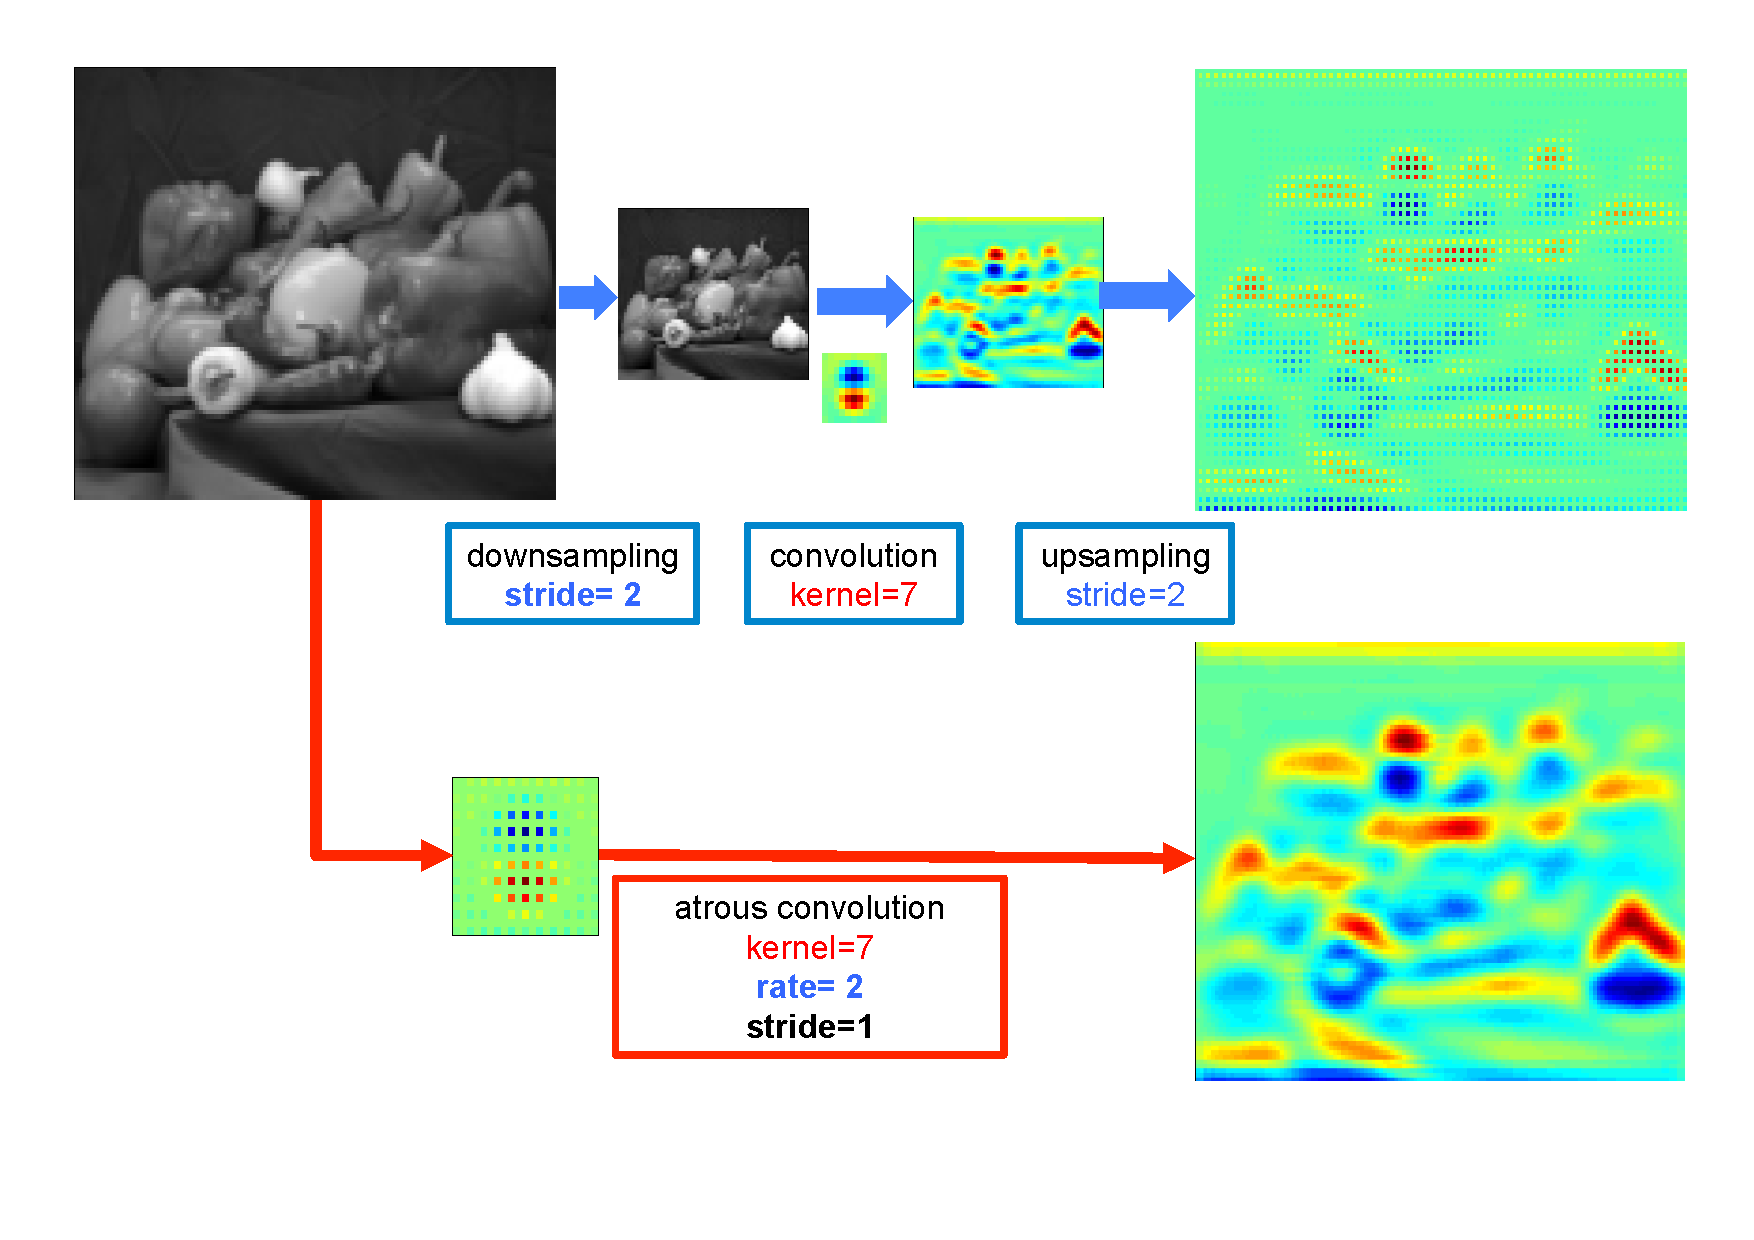
\includegraphics[width=.99 \linewidth]{fig/atrous_slide_rate.pdf}
    	\vspace{-.9cm}
    \end{tabular}
   \caption{Illustration of atrous convolution in 2-D. Top row: sparse feature
   	extraction with standard convolution on a low resolution input feature map.
   	Bottom row: Dense feature extraction with atrous convolution with rate $r = 2$,
   	applied on a high resolution input feature map.}
    \label{fig:hole2d}
   \end{figure}

In the context of DCNNs one can use  atrous convolution in a chain of layers,
 effectively allowing us to compute the final DCNN network responses at an
arbitrarily high resolution. For example, in order to double the spatial density
of computed feature responses in the VGG-16 or ResNet-101 networks, we find the
last pooling or convolutional layer that decreases resolution ('pool5' or 'conv5\_1'
respectively), set its stride to 1 to avoid signal decimation, and replace all
subsequent convolutional layers with atrous convolutional layers having rate
$r = 2$. 
Pushing this approach all the
way through the network could allow us to compute feature responses at the original image
resolution, but this ends up being too
costly. We have adopted instead a hybrid approach that strikes a
good efficiency/accuracy trade-off, using atrous convolution to increase by a
factor of 4 the density of computed feature maps, followed by fast bilinear
interpolation by an additional factor of 8 to
recover feature maps at the original image resolution. Bilinear interpolation
is sufficient in this setting because the class score maps (corresponding to
log-probabilities) are quite smooth, as illustrated in
\figref{fig:score-maps}. Unlike the deconvolutional approach adopted by
\cite{long2014fully}, the proposed approach converts image classification
networks into dense feature extractors without requiring learning any extra
parameters, leading to faster DCNN training in practice. 

Atrous convolution also allows us to arbitrarily enlarge the \emph{field-of-view} of
filters at any DCNN layer.
State-of-the-art DCNNs typically employ spatially small
convolution kernels (typically \by{3}{3}) in order to keep both computation and
number of parameters contained. Atrous convolution with rate $r$ introduces
$r-1$ zeros between consecutive filter values, effectively enlarging the kernel
size of a \by{k}{k} filter to $k_e = k + (k-1)(r-1)$ without increasing the
number of parameters or the amount of computation. It thus offers an efficient
mechanism to control the field-of-view and finds the best trade-off between
accurate localization (small field-of-view) and context assimilation (large
field-of-view). We have successfully experimented with this technique:
Our DeepLab-LargeFOV model variant \cite{chen2014semantic} employs atrous
convolution with rate $r = 12$ in VGG-16 `fc6' layer with significant
performance gains, as detailed in Section~\ref{sec:experiments}.

Turning to implementation aspects, 
there are two efficient ways to  perform atrous convolution. The first
is to implicitly upsample the filters by inserting holes (zeros), or
equivalently sparsely sample the input feature maps \cite{holschneider1989real}.
We implemented this in our earlier work \cite{papandreou2014untangling,
 chen2014semantic}, followed by \cite{yu2015multi}, within the Caffe framework
\cite{jia2014caffe} by adding to the \textsl{im2col} function (it extracts
vectorized patches from multi-channel feature maps) the option to sparsely
sample the underlying feature maps. The second method, originally proposed by
\cite{shensa1992discrete} and used in \cite{giusti2013fast, sermanet2013overfeat}
is to subsample the input feature map by a factor equal to the atrous
convolution rate $r$, deinterlacing it to produce $r^2$ reduced resolution maps,
one for each of the $\by{r}{r}$ possible shifts. This is followed by applying
standard convolution to these intermediate feature maps and reinterlacing them
to the original image resolution. By reducing atrous convolution into regular
convolution, it allows us to use off-the-shelf highly optimized convolution
routines. We have implemented the second approach into the TensorFlow framework
\cite{abadi2016tensorflow}.

%% When applying networks designed for image classification in a fully
%% convolutional fashion for dense prediction tasks, one converts the last fully
%% connected layers into convolutional ones \cite{long2014fully}. This implies
%% that the network spends a much larger fraction of computation in its last
%% few layers, making them the computational bottleneck during both training
%% and evaluation. We have found that we can significantly accelerate a fully
%% convolutional version of the VGG-16 network and at the same time reduce its
%% memory footprint by making two key changes: (1) Thinning the activation maps
%% in the last two hidden layers by a factor of 4, by retaining a random subset
%% of 1,024 out of the original 4,096 filters. (2) Reducing the filter size of
%% the first fully connected layer down to \by{3}{3} (or \by{4}{4}) by
%% subsampling the original \by{7}{7} filters. These changes significantly
%% increase the computational efficiency of our model.

\subsection{Multiscale Image Representations using Atrous Spatial Pyramid Pooling}

DCNNs have shown a remarkable
ability to implicitly represent scale, simply by being trained on datasets that
contain objects of varying size. Still, explicitly accounting for object scale
can improve the DCNN's ability to successfully handle both
large and small objects \cite{papandreou2014untangling}.

We have experimented with two approaches to handling
 scale variability in semantic segmentation.
The first approach amounts to standard multiscale
processing \cite{chen2015attention, kokkinos2016pushing}. We extract DCNN score
maps from multiple (three in our experiments) rescaled versions of the original
image using parallel DCNN branches that share the same parameters. To produce
the final result, we bilinearly interpolate the feature maps from the parallel
DCNN branches to the original image resolution and fuse them, by taking at each
position the maximum response across the different scales. We do this both
during training and testing. Multiscale processing significantly improves
performance, but at the cost of computing feature responses at all DCNN layers for
multiple scales of input. 

The second approach is inspired by the success of the R-CNN spatial pyramid pooling method of \cite{he2014spatial},
which showed that regions of an arbitrary scale can be accurately and efficiently classified by resampling 
convolutional features extracted at a single scale.
 We have implemented a variant of their scheme which uses multiple
parallel atrous convolutional layers with different sampling rates. The features extracted for each sampling
rate are further processed in separate branches and fused to generate the final
result. The proposed ``atrous spatial pyramid pooling'' (DeepLab-ASPP) approach
generalizes our DeepLab-LargeFOV variant and is illustrated in \figref{fig:aspp_fov}.

%%  for the VGG-16 network, where ASPP is applied to the `pool5' features,
%% delivering the input to layer `fc6'.
%%  Another related approach has been successfully pursued by \cite{yu2015multi}: they
%% employ a cascade of serially connected atrous convolutional layers with
%% increasing rate parameters on top of the class score maps, which they show to be
%% effective at capturing multiscale context.

\begin{figure}[!t]
  \centering
  \scalebox{1}{
  \begin{tabular}{c}
    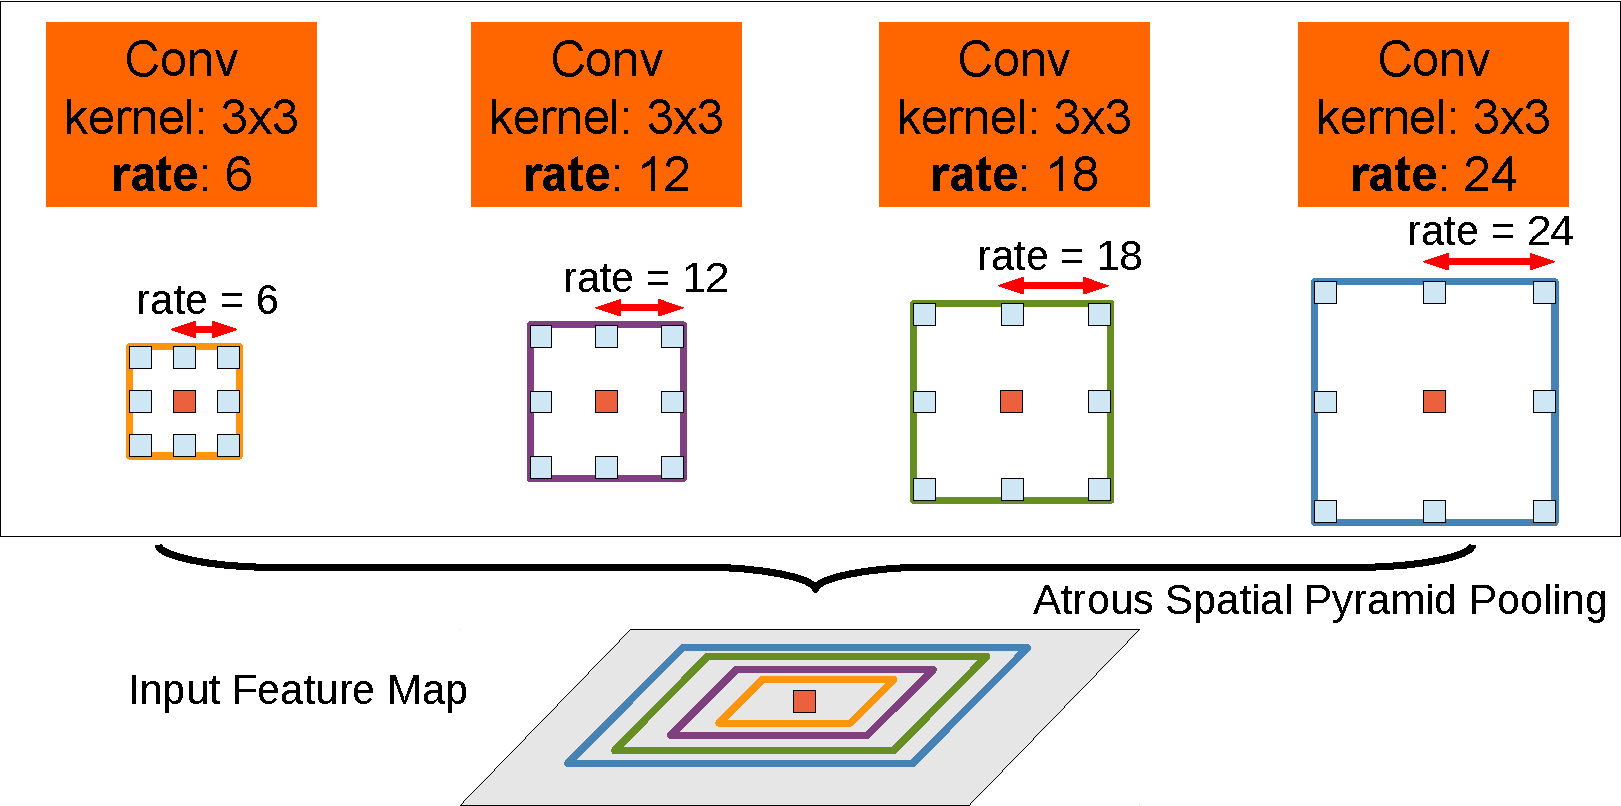
\includegraphics[height=4.5cm]{./fig/spm/aspp2.pdf} \\
  \end{tabular}
  }
  \caption{Atrous Spatial Pyramid Pooling (ASPP). To classify the center pixel (orange),
    ASPP exploits multi-scale features by employing multiple parallel filters with
    different rates. The effective Field-Of-Views are shown in different colors.}
  \label{fig:aspp_fov}
\end{figure}

\subsection{Structured Prediction with Fully-Connected Conditional Random Fields for Accurate Boundary Recovery}
\label{sec:boundary-recovery}

A trade-off between localization accuracy and classification performance seems to be inherent in DCNNs:
deeper models with multiple max-pooling layers have
proven most successful in classification tasks, however the increased
invariance and the large receptive fields of top-level nodes can only yield smooth responses.
%\label{sec:local-chal}
As illustrated in \figref{fig:score-maps}, DCNN score maps can
 predict the presence and rough position of objects but
cannot really delineate their borders. 

Previous work has pursued two directions to address this localization challenge.
The first approach is to harness information from multiple layers in the
convolutional network in order to better estimate the object boundaries
\cite{hariharan2014hypercolumns, long2014fully, eigen2014predicting}. The
second  is to employ a super-pixel representation, essentially
delegating the localization task to a low-level segmentation method
\cite{mostajabi2014feedforward}.

%We have also
%pursued a hybrid approach in which we combine the proposed fully-connected CRF
%method with our own variant of multi-scale prediction. This combined approach
%yields a further performance improvement, as discussed in
%Section~\ref{sec:multiscale}.

%\textbf{Fully-Connected Conditional Random Fields for Accurate Localization}
%\label{sec:dense-crf}

We pursue an alternative direction based on coupling the recognition
capacity of DCNNs and the fine-grained localization accuracy of fully connected
CRFs and show that it is remarkably successful in addressing the localization
challenge, producing accurate semantic segmentation results and recovering
object boundaries at a level of detail that is well beyond the reach of existing
methods. This direction has been extended by several follow-up papers
\cite{papandreou2015weakly, schwing2015fully, zheng2015conditional,
  dai2015boxsup, noh2015learning, liu2015semantic, lin2015efficient,
  chen2015attention, chen2015semantic}, since the first version of our work
was published \cite{chen2014semantic}.

\begin{figure}[t]
  \centering
  \begin{tabular}{c c c c c}
    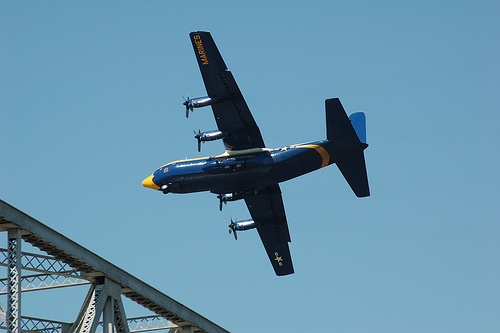
\includegraphics[width=0.16\linewidth]{fig/mean_field_illustration/2007_007470.jpg} & 
    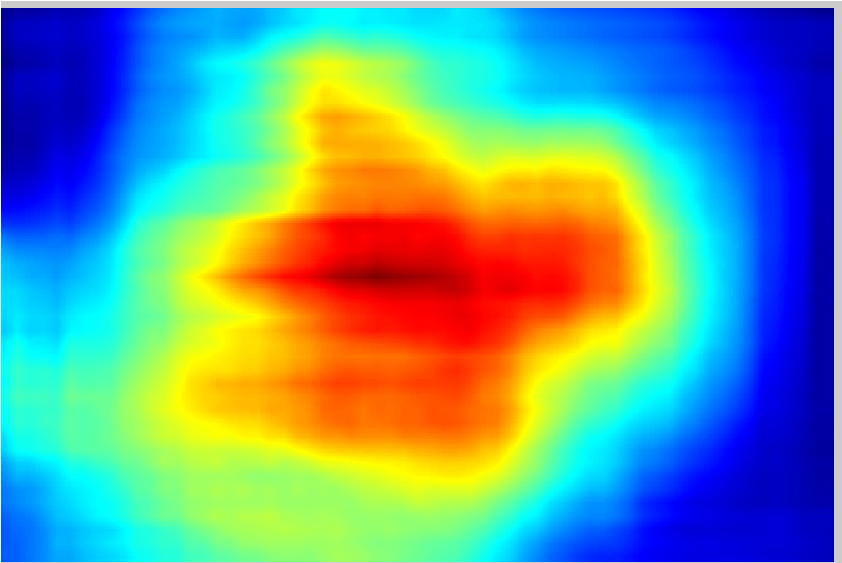
\includegraphics[width=0.16\linewidth]{fig/mean_field_illustration/Score_Class1_Itr0.pdf} &
    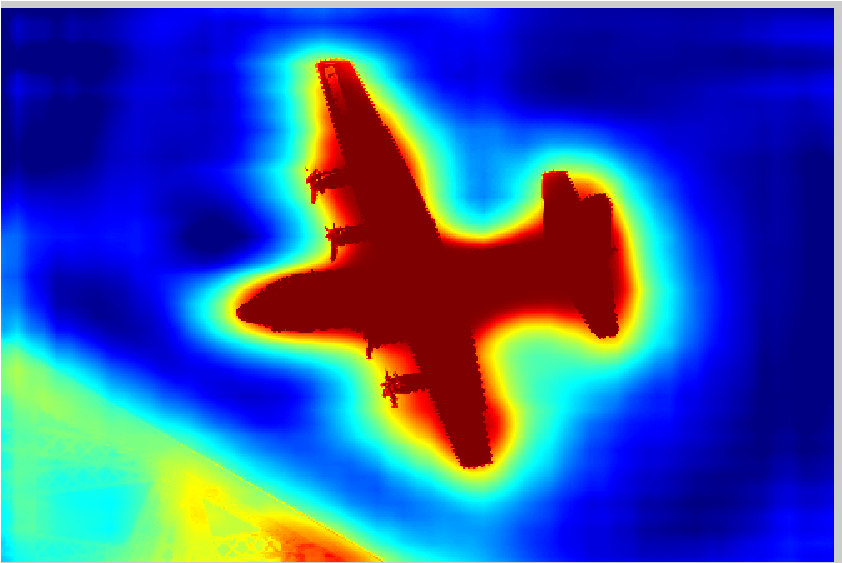
\includegraphics[width=0.16\linewidth]{fig/mean_field_illustration/Score_Class1_Itr1.pdf} & 
    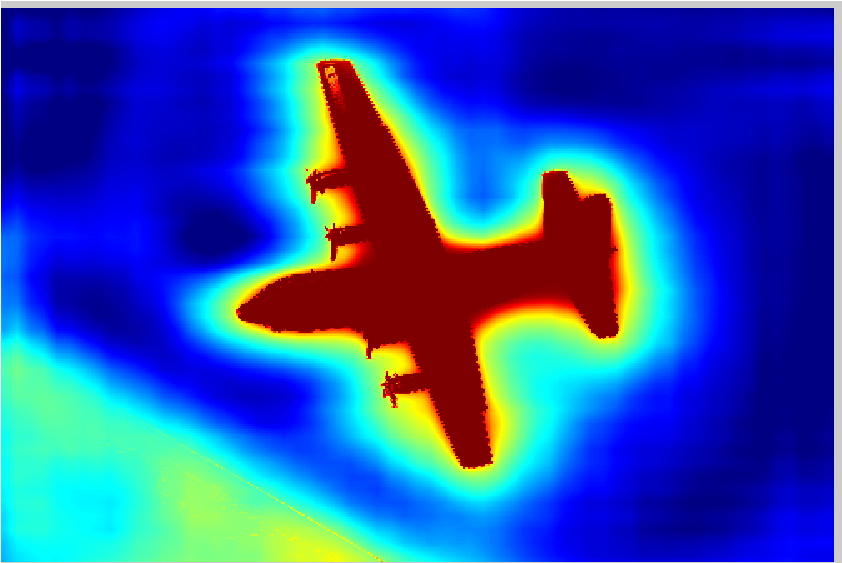
\includegraphics[width=0.16\linewidth]{fig/mean_field_illustration/Score_Class1_Itr2.pdf} & 
    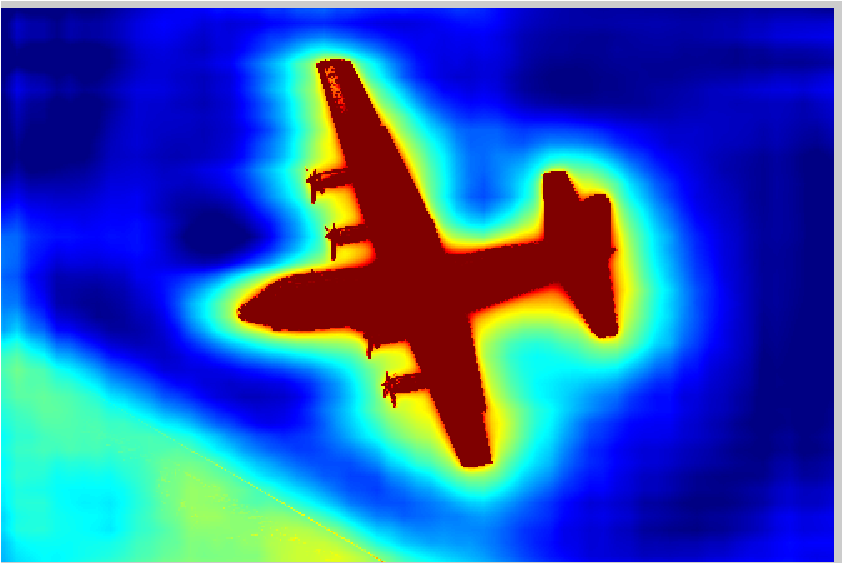
\includegraphics[width=0.16\linewidth]{fig/mean_field_illustration/Score_Class1_Itr10.pdf} \\
    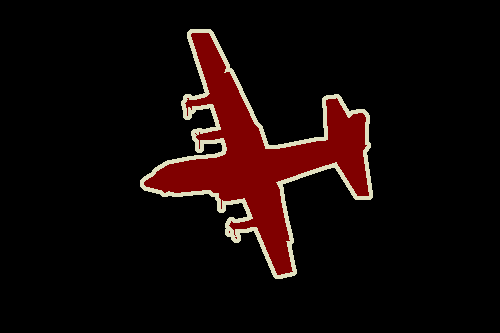
\includegraphics[width=0.16\linewidth]{fig/mean_field_illustration/2007_007470.png} & 
    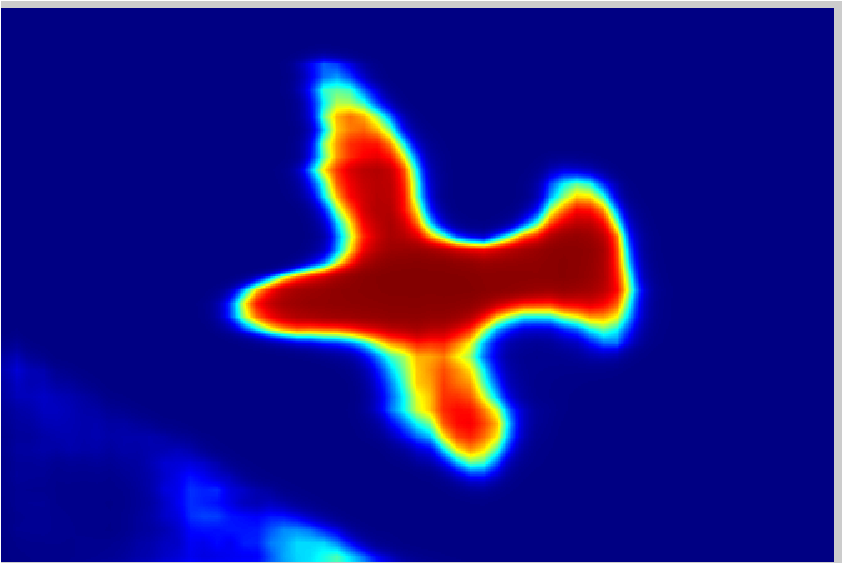
\includegraphics[width=0.16\linewidth]{fig/mean_field_illustration/Belief_Class1_Itr0.pdf} & 
    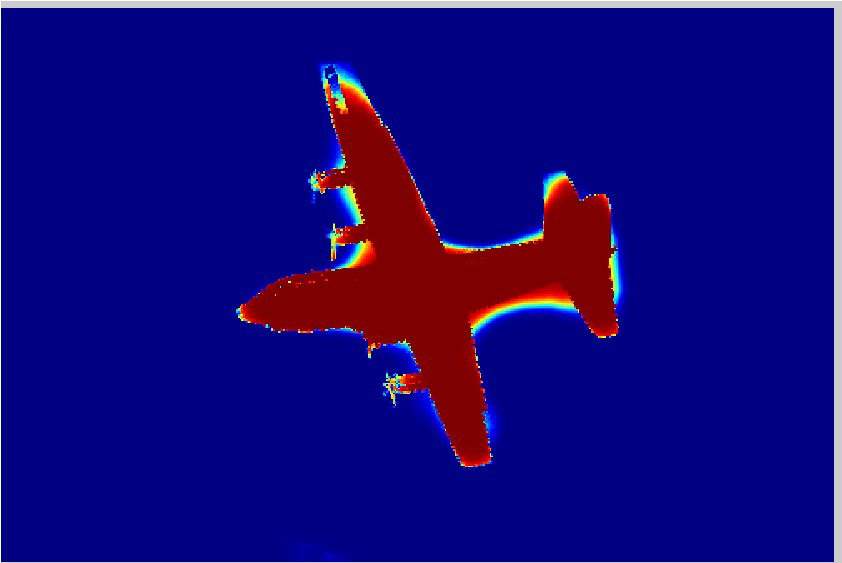
\includegraphics[width=0.16\linewidth]{fig/mean_field_illustration/Belief_Class1_Itr1.pdf} & 
    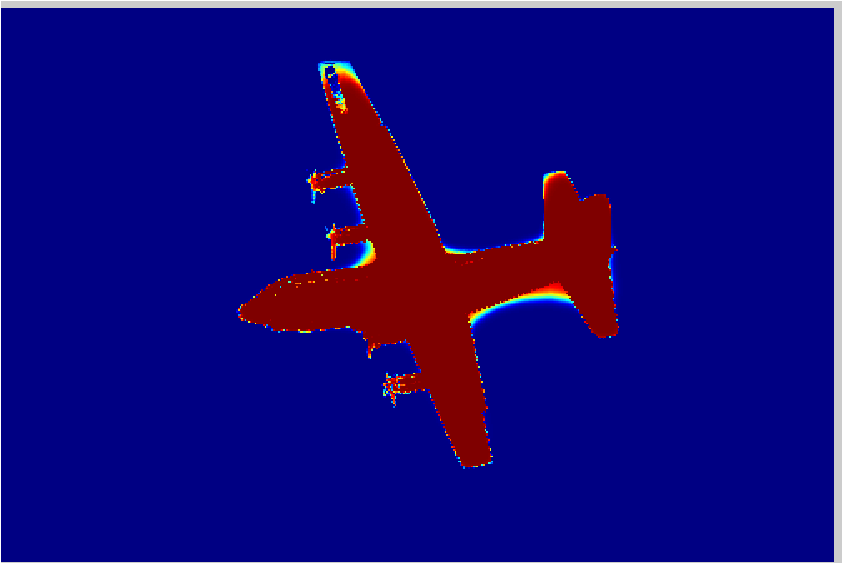
\includegraphics[width=0.16\linewidth]{fig/mean_field_illustration/Belief_Class1_Itr2.pdf} & 
    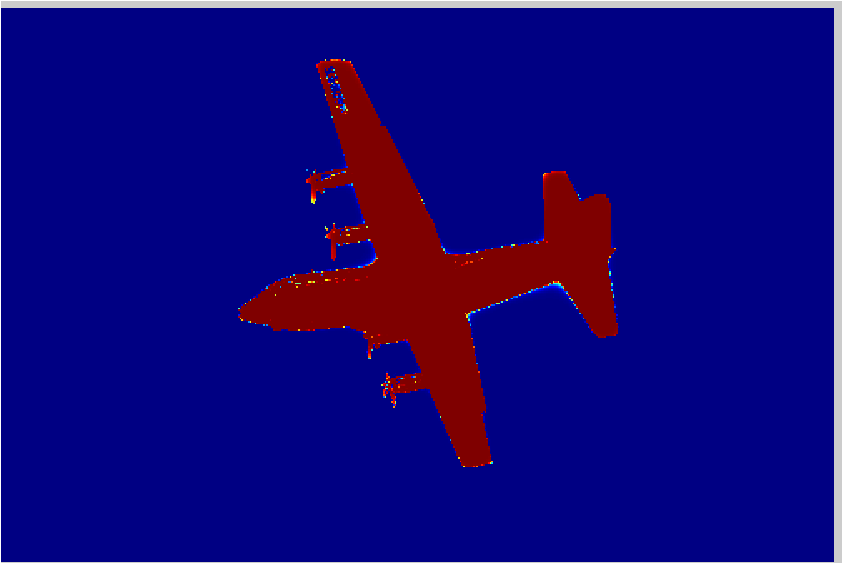
\includegraphics[width=0.16\linewidth]{fig/mean_field_illustration/Belief_Class1_Itr10.pdf} \\
    {\tiny Image/G.T.} & {\tiny DCNN output} & {\tiny CRF Iteration 1} & {\tiny CRF Iteration 2} & {\tiny CRF Iteration 10} \\
  \end{tabular}
  \caption{Score map (input before softmax function) and belief map (output of
    softmax function) for Aeroplane. We show the score (1st row) and belief (2nd row)
    maps after each mean field iteration. The output of last DCNN layer is used as
    input to the mean field inference.}
  \label{fig:score-maps}
\end{figure}

Traditionally, conditional random fields (CRFs) have been employed to smooth
noisy segmentation maps \cite{rother2004grabcut, kohli2009robust}. Typically
these models  couple neighboring nodes, favoring
same-label assignments to spatially proximal pixels. Qualitatively, the
primary function of these short-range CRFs is to clean up the spurious
predictions of weak classifiers built on top of local hand-engineered features.

Compared to these weaker classifiers, modern DCNN architectures such as
the one we use in this work produce score maps and semantic label
predictions which are qualitatively different. As illustrated in
\figref{fig:score-maps}, the score maps are typically quite smooth and
produce homogeneous classification results. In this regime, using short-range
CRFs can be detrimental, as our goal should be to recover detailed local
structure rather than further smooth it. Using contrast-sensitive potentials
\cite{rother2004grabcut} in conjunction to local-range CRFs can potentially
improve localization but still miss thin-structures and typically requires
solving an expensive discrete optimization problem.

To overcome these limitations of short-range CRFs, we integrate into our system
the fully connected CRF model of \cite{krahenbuhl2011efficient}. The model
employs the energy function
\begin{align}
  E(\boldsymbol{x}) = \sum_i \theta_i(x_i) + \sum_{ij} \theta_{ij}(x_i, x_j)
\end{align}
where $\boldsymbol{x}$ is the label assignment for pixels. We use as unary
potential $\theta_i(x_i) = - \log P(x_i)$, where $P(x_i)$ is the label
assignment probability at pixel $i$ as computed by a DCNN. The pairwise
potential has a form that allows for efficient inference while using a fully-connected graph, i.e.
when  connecting 
all pairs of image pixels, $i,j$. In particular, as in \cite{krahenbuhl2011efficient},  we use the following expression:
\begin{gather}
 \hspace{-.2cm}\theta_{ij}(x_i, x_j) \!=\! \mu(x_i,x_j)\!\left[w_1 \exp \Big(\!-\!\frac{||p_i-p_j||^2}{2\sigma_\alpha^2} \!-\!\frac{||I_i-I_j||^2}{2\sigma_\beta^2}\! \Big)\right. \nonumber\\
\left. + w_2 \exp \Big(-\frac{||p_i-p_j||^2}{2\sigma_\gamma^2}\Big)\right]\label{eq:fully_crf}
\end{gather}
where
$\mu(x_i,x_j)= 1 \text{ if } x_i \neq x_j$, and zero otherwise, which, as in the Potts model, means that only nodes with distinct labels are penalized.  The remaining expression uses two Gaussian kernels in different feature spaces; the first, `bilateral' kernel
depends on both pixel positions (denoted as $p$) and
RGB color (denoted as $I$), and the second kernel only depends on pixel
positions. The hyper parameters $\sigma_\alpha$, $\sigma_\beta$ and
$\sigma_\gamma$ control the scale of Gaussian kernels. The  first kernel forces pixels with similar color and position to have similar labels, while the second kernel only considers spatial proximity when enforcing smoothness. 

% labels among pixels 
%when 
% (Potts model).
%Each Gaussian kernel $k^m$ depends on features (denoted as
%$\boldsymbol{f}$) extracted for pixel $i$ and $j$ and is weighted by
%parameter $w_m$. Specifically, we adopt bilateral position and color kernels
%\begin{align}
%  \label{eq:fully_crf}
%  w_1 \exp \Big(-\frac{||p_i-p_j||^2}{2\sigma_\alpha^2} -\frac{||I_i-I_j||^2}{2\sigma_\beta^2} \Big) \nonumber \\
%  + w_2 \exp \Big(-\frac{||p_i-p_j||^2}{2\sigma_\gamma^2}\Big)
%\end{align}
%where the first kernel 

Crucially, this model is amenable to efficient approximate probabilistic
inference \cite{krahenbuhl2011efficient}. The message passing updates under a
fully decomposable mean field approximation $b(\boldsymbol{x}) = \prod_i
b_i(x_i)$ can be expressed as Gaussian convolutions in bilateral
space. High-dimensional filtering algorithms \cite{adams2010fast}
significantly speed-up this computation resulting in an algorithm that is very
fast in practice, requiring less that 0.5 sec on average for Pascal VOC images using the
publicly available implementation of \cite{krahenbuhl2011efficient}.
